\documentclass{beamer}
\title{Evaluation of Self-improved prompts}
\author{Deebakkarthi Chinnasame Rani}
\date{2026-11-24}

\usepackage{graphicx}
\usepackage{booktabs}
\usepackage{tabularx}

\begin{document}
\frame{\titlepage}

\begin{frame}{Motivation}
\begin{itemize}
\item When comparing
\textit{pasting an RTL file in its entirity} vs \textit{Using} \texttt{Read()},
I noticed that \texttt{Read()} performed much better.

\item Before moving on techniques such as
\textit{using LTL, RAG, Knowledge graphs, etc...}, I wanted to see the limits
of plain prompt engineering and some feedback mechanism.
\end{itemize}
\end{frame}

\begin{frame}{Flow}
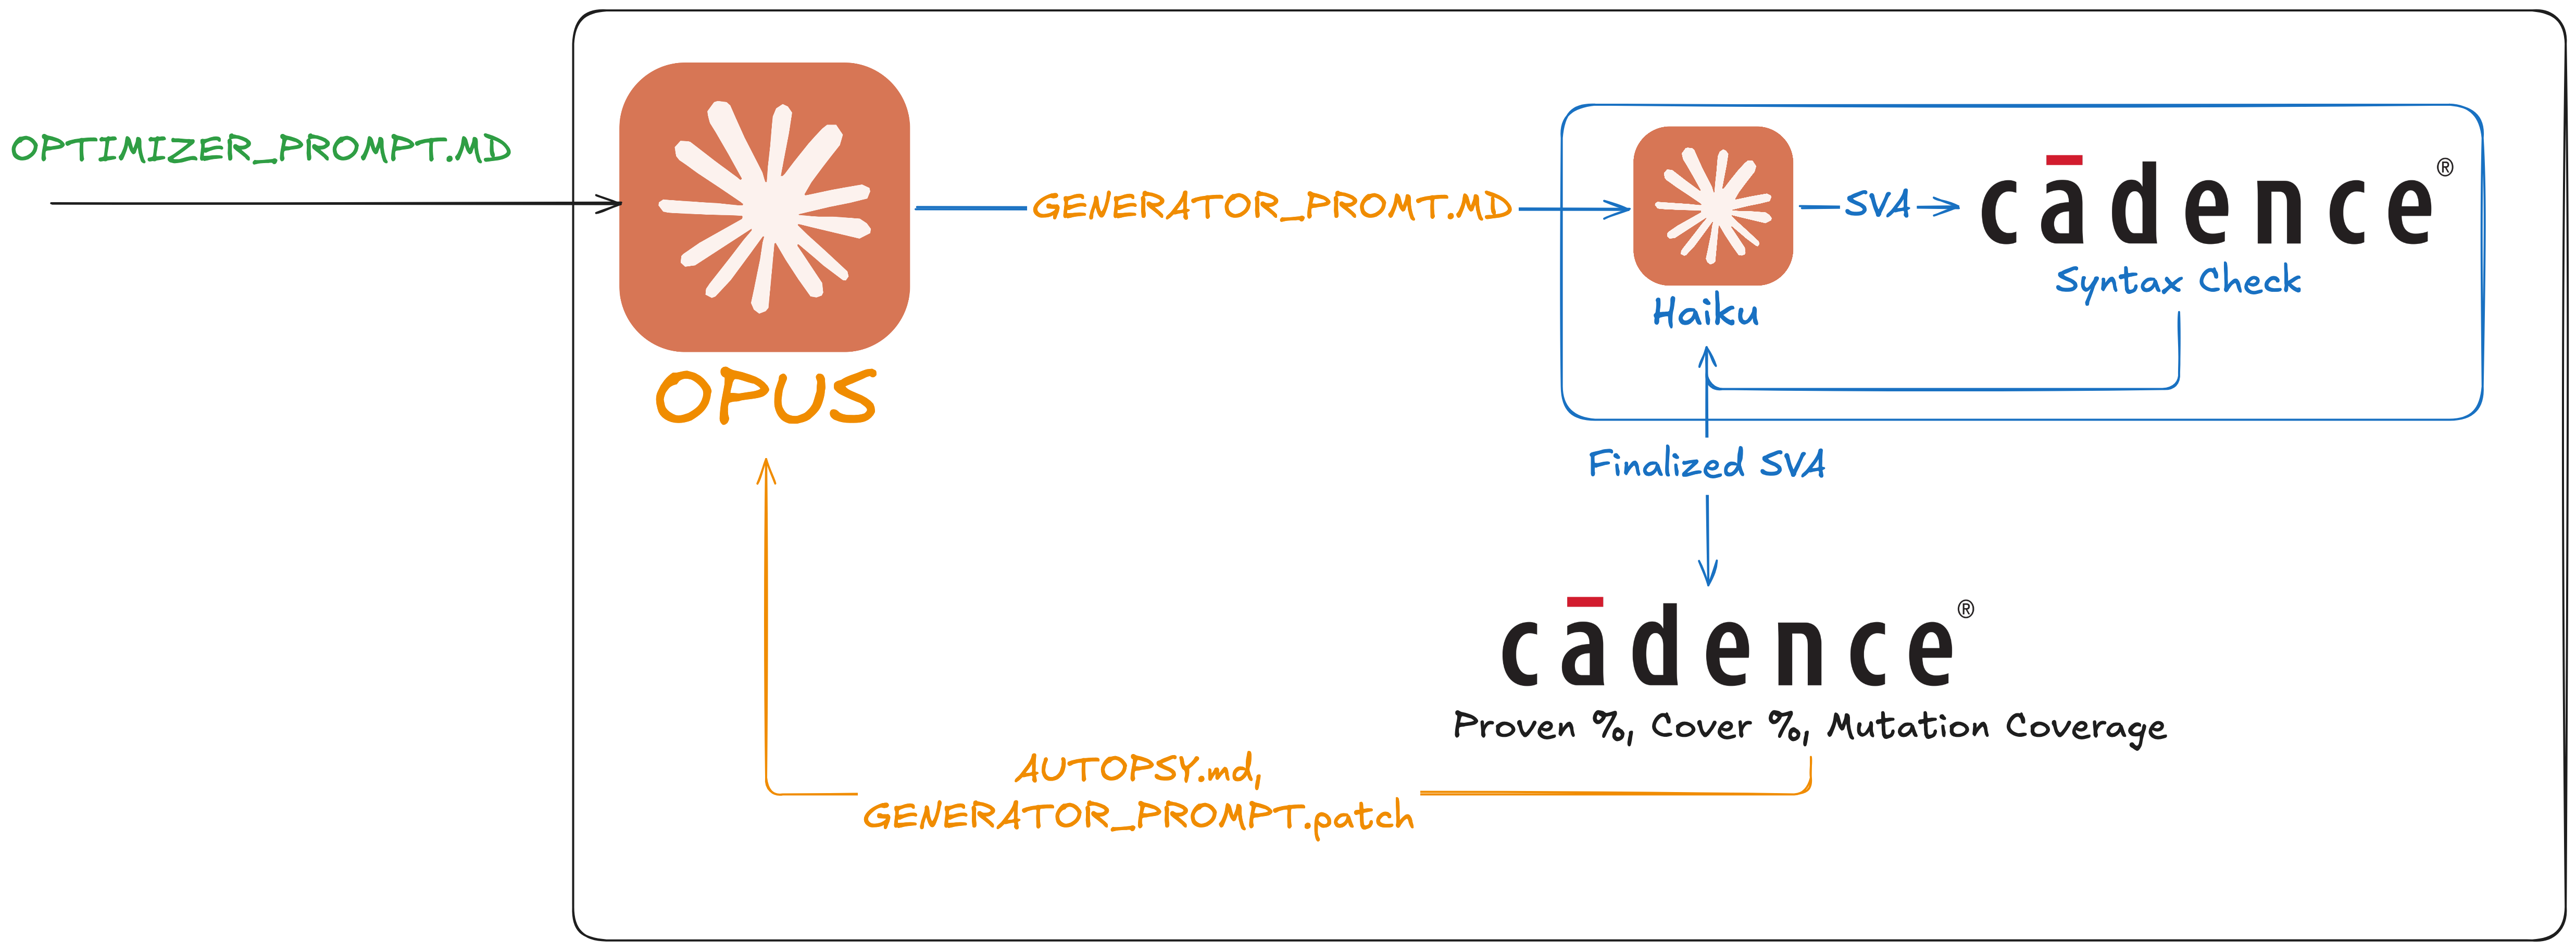
\includegraphics[width=\textwidth]{flow}
\end{frame}

\begin{frame}{Training on \texttt{onewire}}
% Please add the following required packages to your document preamble:
% \usepackage{booktabs}
\begin{table}[]
\centering
\begin{tabular}{|l|l|}
\toprule
\multicolumn{1}{|c|}{\textbf{Iteration}} & \multicolumn{1}{c|}{\textbf{Proven \%}} \\ \midrule
1                                        & 69.5                                    \\ \midrule
2                                        & 75.0                                    \\ \midrule
3                                        & 88.0                                    \\ \midrule
4                                        & 94.6                                    \\ \midrule
5                                        & 95.4                                    \\ \bottomrule
\end{tabular}
\end{table}
\end{frame}

\begin{frame}{Testing on \texttt{i2c}}
\begin{table}[]
\centering
\begin{tabular}{|l|l|l|}
\toprule
Model  & Proven/ Total (Proven \%) & Formal Mutation Coverage \\ \midrule
\texttt{haiku}  & 37/45 (82.2\%)            & 102/806 (12.7\%)         \\ \midrule
\texttt{sonnet} & 48/49  (98.0\%)           & 111/806 (13.8\%)         \\ \midrule
\texttt{opus}   & 135/209 (64.6\%)          & 518/806 (64.3\%)         \\ \bottomrule
\end{tabular}
\end{table}
\end{frame}

\begin{frame}{Comparison vs \texttt{AssertLLM2}'s default prompt}
% Please add the following required packages to your document preamble:
% \usepackage{booktabs}
% \usepackage{tabularx}
\begin{table}[]
\centering
\begin{tabularx}{\linewidth}{|l|>{\raggedright\arraybackslash}X|l|}
\toprule
Prompt     & Proven/ Total (Proven \%) & Formal Mutation Coverage \\ \midrule
AssertLLM2 & 46/55  (83.6\%)           & 118/806 (14.64\%)        \\ \midrule
Ours       & 135/209 (64.6\%)          & 518/806 (64.3\%)         \\ \bottomrule
\end{tabularx}
\end{table}
\end{frame}

\end{document}
